\chapter{Computing thermal conductivity} 

\label{Chapter2} 

In Chapter~\ref{Chapter1}, I introduced the key concepts surrounding this study. I will be investigating the magnitude of thermal conductivity throughout the deep Earth, considering the effect of physical conditions and Fe impurities. I will be using computational approaches to access this parameter, as experiments are difficult to perfrom in the regime I require. 

Part of computing results is ensuring the simulations are running faithfully to the material of interest and the physical processes that operate in bulk materials. In this chapter I introduce the background to calculating conductivity through simulation, and show fundamental system setup and parameter convergence. 

The following chapters apply theory introduced here to investigate how conductivity is affected by; system shape and size, and adding impurities to an otherwise regular crystal structure.

%-----------------------------------------------------------
\section{Atomic-scale modelling}
%-----------------------------------------------------------

!!! THIS SECTION HAS REDUNDANCY WITH ABOVE CHAPTER INTRO SPIEL

!!! PROBABLY REVISE HEAVILY

Knowledge of thermal conductivity is important for modelling the deep earth, but can not be measured experimentally at core mantle boundary conditions. Atomic scale simulations sidestep experimental limitations, but system size must be chosen carefully in order to determine accurate conductivity values. 

A range of atomic scale simulation methods are available to determine the lattice thermal conductivity of materials. These are invaluable for calculating thermal conductivity at conditions of which experiments are difficult, e.g. the extreme conditions found in the Earth's lower mantle (pressures and temperatures up to 136~GPa and 4000~K at the core-mantle boundary). 

%---------------------------------------
\subsection{Computational approaches (for modelling atoms...?)}
%---------------------------------------

Before you can calculate material properties of interest, you need to determine how the atoms will interact with one another in your system. I do not mean the magnitude of the interactions or the parameters you choose to replicate a material, but the specific theoretical approach of atomic-scale modelling. There are multiple regimes for doing so, a couple of which are described below.

%-------------------
\subsubsection{Molecular dynamics}
%-------------------

In a moldecular dynamics (MD) calculation, atoms in a simulation cell have masses, velocities, and forces acting between them. At each computational timestep the net force on each atom is calculated from all the other atoms. Accelerations are then calculated from Newton's second law of motion, which are used to update the velocities and positions of the atoms. The process is repeated, iteratively updating parameters every timestep. At zero temperature, a parameter such as unit cell volume will converge, but this is not true when finite temperatures are considered. Temperature fluctuations mean cell volume will constantly change, regardless of simulation length. The solution is to take the cumulative average over many timesteps, which converges eventually.

!!! FLOWCHART FIGURE, MD TIMESTEP PROCESS?

%-------------------
\subsubsection{Lattice dynamics}
%-------------------

An alternative approach to MD is lattice dynamics (LD),where the response of all atoms to the motion of one is considered. Each atom in the simualtion cell is perturbed in turn, the motions and response of the other atoms stored  in a 3 by 3 tensor for each atom pairing. The tensor takes significant time to compute compared to a single MD timestep, but can be used to calculate various material properties once obtained. The focus of this study will be on MD approaches, but LD results from literature will be reviewed for comparison.

!!! ADD A REFERENCE AND FORGET ABOUT IT?

!!! DO I NEED TO SAY WHY I AM NOT USING LD? WHY AM I NOT USING LD!?














%---------------------------------------
\subsection{Calculating atomic interactions}
%---------------------------------------

!!! ADD INTRO SPIEL HERE

%-------------------
\subsubsection{Density functional theory}
%-------------------

Density functional theory (DFT) is a way of determining accurate interatomic forces. The properties of the electrons are considered along with the nuclei, which increases the computational cost and simulation run time. This additionally limits the size of systems, or number of atoms (on the order of thousands), that can be considered. Calculating from first principles in this manner should only be considered if you know the system parameters for converged results, and they can be completed on a suitable timescale. I will be opting for a different approach, as I wish to investigate a large amount of big systems systems, potentially for multiple compositional variations.

!!! ANY OTHER ALTERNATIVE APPROACHES THAT NEED TO GO HERE?

%-------------------
\subsubsection{Classical interatomic potentials}
%-------------------

The alternative to DFT is to use empirically-derived potentials to calculate the interatomic forces. Whereas calculating from first principles considers the interactions of atoms and their outer shell electrons, interatomic potentials use an approximation of the electronic potential component (i.e. a classical atomic model). 

Systems on the order of millions of atoms can be considered with atomic potentials, due to significantly reduced computational cost compared to DFT. The trade-off is accuracy however, which is controlled by the characteristics of the employed potential. These potentials are set up to reproduce a set of experimental results, but the is no certainty they reflect true values outside their calibrated range of conditions. A realsitic model reproduces the structural, elastic, and thermal properties of a material. A common feature of classical potentials is to underestimate the diagonal terms of the elastic constant tensor, and overestimate the off-diagonal, where the discrepancy increases with pressure \citep{Chen2012}.

%-------------------
\subsubsection{Oganov's \bdgs potential}
%-------------------

The interatomic potential I will be using  was developed by \citet{Oganov2000}. Many potentials exist for \mgsios perovskite, but the aforementioned is robust up to lower mantle pressures and temperatures. The interatomic potential function includes ionic, covalent, and van der Waals components. The dominant long-range term is the Coulomb interaction, and the short-range interactions are described using a Buckingham potential with the Born-Mayer potential, and a $C/r^{6}$ van der Waals term. The equation for pair-wise potential (summed for potential energy of the system) takes the form
%
\begin{equation}
V_{ij}^{\mathrm{Buck}}
= \frac{1}{4 \pi \epsilon_{0}} 
\frac{q_{i} q_{j}}{r_{ij}} 
+ b_{ij}\ exp\left ( \frac{-r_{ij}}{\rho_{ij}} \right )
- \frac{c_{ij}}{{r_{ij}}^{6}} \  ,
\label{eq.buck}
\end{equation}
%
where $q_{i}$ and $q_{j}$ are the charges of atoms $i$ and $j$, $r_{ij}$ is the distance between them, $b_{ij}$ is the pre-exponential repulsive parameter for the pair, $\rho_{ij}$ is the repulsion exponent, and $c_{ij}$ is the van der Waals parameter.
There are three sets of these paramters, for each of the interacting atomic pairs (shown in Table~\ref{tab.oganov}). The charges for Mg, Si, and O atoms are $1.9104$, $2.9043$, and $-1.6049$, respectively.
%
\begin{table}[h]
\centering
\caption[CONTENTS BIT]{\label{tab.oganov}Parameters used to define \citet{Oganov2000}'s \mgsios perovskite potential.}
\begin{tabular}{clll} 
Bond $ij$ & $b_{ij}$ (eV)  & $\rho_{ij}$ (\AA) & $c_{ij}$ (eV.\AA$^{6}$) \\ \hline
Mg-O        & 1041.435        & 0.2866                 & 0                \\
Si-O          & 1137.028        & 0.2827                 & 0                \\
O-O          & 2023.800        & 0.2674                  & 13.83         \\ \hline       
\end{tabular}
\end{table}



%-------------------
\subsubsection{SETTING UP POTENTIAL CUTOFFS}
%-------------------

Part of applying classical potentials is setting up the distance over which they act, the maximum seperation between two atoms before they are not paired for force calculation. Too small a cut-off distance, and the material is not being replicated faithfully. Too large a cut-off, you are performing more calculations than you need, and will increase computation time. The potential between two atoms is inversely proportional to their separation (see Eq. \ref{eq.buck}), ``cutting off'' in this manner is acceptable when the value is tending towards zero with large interatomic distance. I consider two cut-off distances, for both the Coulombic and the Buckingham interactions (the former have a larger value than the latter).

 !!! BUT WHAT DID I DECIDE ON THOUGH 
 
% 150527_pressures.xlsx 


%-------------------
\subsubsection{MD ensembles}
%-------------------

!!! EXPAND THIS TOPIC? MOVE UP TO MD SECTION?

There are 3 styles of molecular dynamics ensemble that I will utilise over the course of this project, to perform different kinds of calculations. These are NPT, NVT, and NVE, where N refers to the number of atoms, P to pressure, T to temperature, V to volume, and E to energy. The number of atoms is kept constant in all cases presented here. 

In NPT and NVT simulations, the system is thermostatted to a specified temperature. In NPT a barostat is also set, and the cell volume is allowed to equilibrate with the pressure and temperature conditions. This kind of simulation is performed before calculating parameters like thermal conductivity, in order to recreate conditions like the CMB (i.e. 136~GPa, 4000~K). One cannot simply equilibrate the system at high pressure and then run temperature initialisation, this will introduce an effect of thermal pressure. If this equilibration is performed incorrectly, one might end up with a CMB at 145~GPa for example, ultimately causing conductivity results to be overestimated (as they increase with pressure).

Once the cell is of a suitable volume for the conditions of interest, the temperature of the system (via the velocities of the atoms) can be initialised through computation in the NVT regime. Freedom to control the initial temperature condition is great for studies where repeatability or gathering a sample of data is important. The structure, conditions, and subsequent computation steps don't change, but the result will varying in a given distribution from the random nature of atomic velocities and motion. While pressure is free to change, it will remain constant assuming the aforementioned NPT equilibration is perform to obtain a suitable cell volume. Volume can't change, and temperature is thermostatted, so there are no variations in thermal pressure.

Once a reasonable distribution and steady average temperature are obtained, a system can be computed in the NVE ensemble. For both the direct and Green-Kubo methods I utilise, conductivity results are determined in this regime. The kinetic and potential energies of the atoms are held constant, allowing local temperature variations. The same point about variable pressure applies here as well as with NVT, but an overall consistent average temperature means a similarly average pressure. NVE is used in this was thermostatting can affect the dynamics of the system.

!!! EXPAND THIS TOPIC? MOVE UP TO MD SECTION?









%---------------------------------------
\subsection{Finite-size effects}
%---------------------------------------

Computational techniques are not limited by the reproduction of physical conditions like experiments, this does not mean they are without limitations however. Finite-size effects refer to when the number of atoms or system shape and size affect the computed result, compared to an infinite system. In the case of thermal conductivity, the problem arises when phonons are truncated by boundaries in the simulation cell. As discussed in Chapter~\ref{sec.phonon_explan}, phonons have wave-like properties, including wavelength. 

When a simulation cell is shorter than a phonon's wavelength, that phonon cannot be represented in the system. This will mean a calculation is tending to underestimate conductivity, the phonon population is not being fully represented. Another scenario is if the phonon mean free path is longer than the distance between boundaries in a system, phonon scattering behaviour is not being replicated accurately. This leads to overestimations, where phonons are able to transport heat unimpeded, and conductivity is strongly dependent on system size \citep{Tadano2014}. 

The FSE observed for a material change with thermal conductivity/phonon MFP, and thus are pressure, temperature, and composition sensitive. Long MFPs require larger systems to eliminate FSE (and vice versa) [[[BUT IS THIS TRUE?]]].

This can be a problem when employing DFT calculations, where systems sizes must be kept small to maintain computational efficiency. Testing system size is also a problem, as calculations of large systems must be performed to check convergence of results.

%-------------------
\subsubsection{LAMMPS}
%-------------------

LAMMPS (Large-scale Atomic/Molecular Massively Parallel Simulator) is a classical molecular dynamics code \citep{Plimpton1995}. I will be using it to look at large systems (up to the order of $10^5$ atoms) and assess how size and shape affects results. While calculations using interatomic poternials are not as accurate as those using DFT, a main focus of this work will be on the observations of conductivity magnitude change between systems of varying size. The \wmks result isn't as important as confirming phonon behaviour is not being greatly inhibited. 

While not considered here, the system size parameters I determine for \bdgs at a range of temperatures and pressures could be used in a DFT calculation. This ensures the DFT calculation is using a large enough arrangement of atoms, while providing a useful reliability check for my classical results. 



%-------------------
\subsubsection{Calibration and comparison}
%-------------------

For my calculations to be valid, I have to be able to reproduce other results calculated using the \citet{Oganov2000} potential. \citeauthor{Oganov2000} provide lattice parameters for a unit cell, along with elastic constants and the bulk and shear moduli. I reproduced their results to accpetable accuracy (see Table \ref{tab:oga_pot}, page \pageref{tab:oga_pot}), using LAMMPS and the lattice dynamics code GULP \citep{Gale1997}. Of particular note in this table is the agreement of the static LAMMPS and GULP results, showing the potential has been implemented identically for both codes. With regards to the 300~K results, GULP and LAMMPS differ, but only by around 1\% for each property. The standard error on the LAMMPS values is smaller than the difference with the GULP values, this disparity is caused by the use of lattice dynamics (LD) opposed to molecular dynamics (MD). The GULP (LD) values are believed to be more accurate in this case, 
as 300~K is likely below the Debye temperature for perovskite. Calculations run below this temperature will not accurately recreate the material's thermal properties, due to the inactivity of some phonon modes. This will not be a concern when calculating thermal conductivity, as I will be using temperatures on the order of thousands of Kelvin.

\begin{sidewaystable}[htbp]
\centering
\caption{Comparison of \mgsios perovskite properties calculated using the \citet{Oganov2000} potential at 0~GPa}\vspace{2mm} 

\begin{tabular}{l|l|l|l|l|l}
\hline
Property  &  \citeauthor{Oganov2000} (Static) & GULP (Static) & LAMMPS (Static) & GULP (LD, 300~K) & LAMMPS (MD, 300~K) \\ \hline
a (\AA)                   & 4.7822               & 4.7875            & 4.7875         & 4.8074      & 4.8022	\\ 
b (\AA)                   & 4.8960               & 4.9001            & 4.9002          & 4.9193      & 4.9140	\\ 
c (\AA)   		      & 6.9322               & 6.9366            & 6.9366          & 6.9598      & 6.9530	\\ 
V (\AA$^{3}$)      & 162.31               & 162.73            & 162.73          & 164.59      & 164.08	\\ \hline
C$_{11}$ (GPa)     & 500                   & 507                 & 507               & 492           & 487	\\ 
C$_{22}$ (GPa)     & 509                   & 519                 & 519               & 502           & 498	\\ 
C$_{33}$ (GPa)     & 398                   & 411                 & 411               & 395           & 395	\\ 
C$_{12}$ (GPa)     & 116                   & 125                 & 125               & 117           & 116	\\ 
C$_{13}$ (GPa)     & 210                   & 209                 & 209               & 205           & 201	\\ 
C$_{23}$ (GPa)     & 188                   & 192                 & 192               & 185           & 184	\\ 
C$_{44}$ (GPa)     & 174                   & 177                 & 177               & 172           & 170	\\ 
C$_{55}$ (GPa)     & 189                   & 189                 & 189               & 186           & 184	\\ 
C$_{66}$ (GPa)     & 102                   & 108                 & 108               & 103           & 102	\\ \hline
K$_{H}$ (GPa)  & 270.4                & 276.5              & 276.5            & 266.8        & 269.9	\\ 
G$_{H}$ (GPa)  & 146.3                & 150.1              & 150.0            & 145.2        & 145.7	\\
\hline       
\end{tabular}
\\ \vspace{2mm}
a, b, c, and V represent lattice vectors and unit cell volume. C$_{xx}$ denotes elastic constants. K$_{H}$ and G$_{H}$are the Voigt-Reuss-Hill averaged bulk and shear moduli. The MD LAMMPS elastic constants have standard error on the order of 0.1.
\label{tab:oga_pot}
\end{sidewaystable}

	\par \citet{Ammann2014} used GULP and the \citet{Oganov2000} potential, and provide unit cell lattice parameters for sample lower mantle pressures and temperatures. I reproduced their data to within $\sim$0.1\% (see Table \ref{tab:ammann_comp}, page \pageref{tab:ammann_comp}), the above mentioned difference between LD and MD reducing with increased temperatures.

\begin{sidewaystable}[htbp]
  \centering
  \caption{Comparison of calculated \mgsios peroskite unit cell parameters with \cite{Ammann2014}}\vspace{2mm}
    \begin{tabular}{cc|lll|lll|lll}
    \hline
    \multirow{3}[2]{*}{Pressure (GPa)} & \multirow{3}[2]{*}{Value} & \multicolumn{9}{c}{Lattice parameter (\AA) at a given temperature (K)} \\
          &       &       & 1000  &       &       & 2000  &       &       & 3000  &  \\
          &       & a     & b     & c     & a     & b     & c     & a     & b     & c \\ \hline
    \multirow{4}[2]{*}{20} & My work & 4.7281 & 4.8336 & 6.8215 & 4.7701 & 4.8676 & 6.8670 & 4.8220 & 4.9102 & 6.9127 \\
          & Standard error & 0.0001 & 0.0001 & 0.0001 & 0.0001 & 0.0001 & 0.0001 & 0.0006 & 0.0006 & 0.0006 \\
          & \citeauthor{Ammann2014} & 4.7281 & 4.8342 & 6.8221 & 4.7708 & 4.8685 & 6.8653 & 4.8293 & 4.9169 & 6.9070 \\
          & \% Difference & 0.00  & 0.01  & 0.01  & 0.02  & 0.02  & 0.02  & 0.15  & 0.14  & 0.08 \\ \hline
    \multirow{4}[2]{*}{130} & My work & 4.3787 & 4.5180 & 6.3290 & 4.3985 & 4.5265 & 6.3495 & 4.4191 & 4.5352 & 6.3706 \\
          & Standard error & 0.0001 & 0.0001 & 0.0001 & 0.0001 & 0.0001 & 0.0001 & 0.0001 & 0.0001 & 0.0001 \\
          & \citeauthor{Ammann2014} & 4.3807 & 4.5192 & 6.3236 & 4.4003 & 4.5244 & 6.3438 & 4.4203 & 4.5347 & 6.3691 \\
          & \% Difference & 0.05  & 0.03  & 0.08  & 0.04  & 0.05  & 0.09  & 0.03  & 0.01  & 0.02 \\
    \hline
    \end{tabular} 
\\ \vspace{2mm}
Data produced using LAMMPS is compared with the GULP results of \cite{Ammann2014}, across a range of pressure/temperature conditions. The standard error is calculated from 1E6 timesteps of NVT simulation. The percent difference refers to the variation between my work and \citeauthor{Ammann2014}'s. 
  \label{tab:ammann_comp}%
\end{sidewaystable}%








\pagebreak
















%-----------------------------------------------------------
\section{Computing \tc}
%-----------------------------------------------------------

I will be using two approaches, both utilising classical interatomic potentials, to calculate thermal conductivity throughout this thesis. They will be explained later in this section, and are as follows,

(1) The non-equilbrium molecular dynamics-based ``direct method'', where thermal conductivity is calculated from an imposed heat flux and corresponding temperature gradient via Fourier's Law \citep{Muller-Plathe1997,Nieto-Draghi2013}.

(2) Equilibrium molecular dynamics based on the Green-Kubo relations to determine the thermal conductivity from heat flux fluctuations and their time-dependence \citep{Green1954,Kubo1957,Kubo1966,Schelling2002}. 


\citet{Stackhouse2010} review other methods to compute thermal conductivity, including the above, but also

(3) Anharmonic lattice dynamics \citep{Tang2009}. %(BTE)CHERNATYNSKIY and PHILLPOT 2010?

(4) Combined quasiharmonic lattice dynamics and molecular dynamics method \citep{DeKoker2009}.

!!! Fixed ends? Sinusoidal temperature perturbation?

The Green-Kubo and direct method use the same underlying atomic model, but calculate \tcs differently. They have their own unique system setup procedures, data processing work flows, and finite-size effects. In the following sections, each method will be considered individually, before a review of literature comparing the two, and how I will use them to analyse their FSE.



%---------------------------------------
\subsection{Direct method}
%---------------------------------------
The direct method is the computational implementation of a typical experiment to measure thermal conductivity, using Fourier's law to relate heat flux ($q$) and temperature gradient ($\nabla{T}$) to thermal conductivity ($k$)
%
\begin{equation}
q=-k \nabla{T}\ . 
\label{fourier}
\end{equation}

%-------------------
\subsubsection{System setup}
%-------------------

In the direct method energy is transferred from one group of atoms to another at regular intervals, creating hot and cold regions between which heat flows. This heat transfer process is implemented by taking the velocity of the lowest energy atom in the hot section, and swapping it with the highest energy atom in the cold section \citep{Muller-Plathe1997}. The resultant temperature gradient is measured by calculating the temperature of individual groups of atoms along the direction of the heat flux. Thermal conductivity is equal to the ratio of imposed heat flux to the resulting temperature gradient. This can be shown in a rearranged version of Fourier's law
%
\begin{equation}
k = - \frac{\left \langle J \right \rangle}{\left \langle dT/dx \right \rangle}\ ,
\label{fourier2}  
\end{equation}
%
where $k$ is thermal conductivity, $\left \langle J \right \rangle$ is heat flux through a unit cross-sectional area, and $\left \langle dT/dx \right \rangle$ is the temperature gradient between hot and cold regions. 

Simulation cells tend to be long relative to their cross-sectional area, defined as height by width (see Figure~\ref{fig:cell_dia}). Cell boundaries are periodic and the hot and cold sections are half the cell length apart, meaning heat flows in both directions from hot to cold (one of which is across the length-end periodic boundary). This results in two similar temperature gradients which can be averaged.

\begin{figure}[h]
  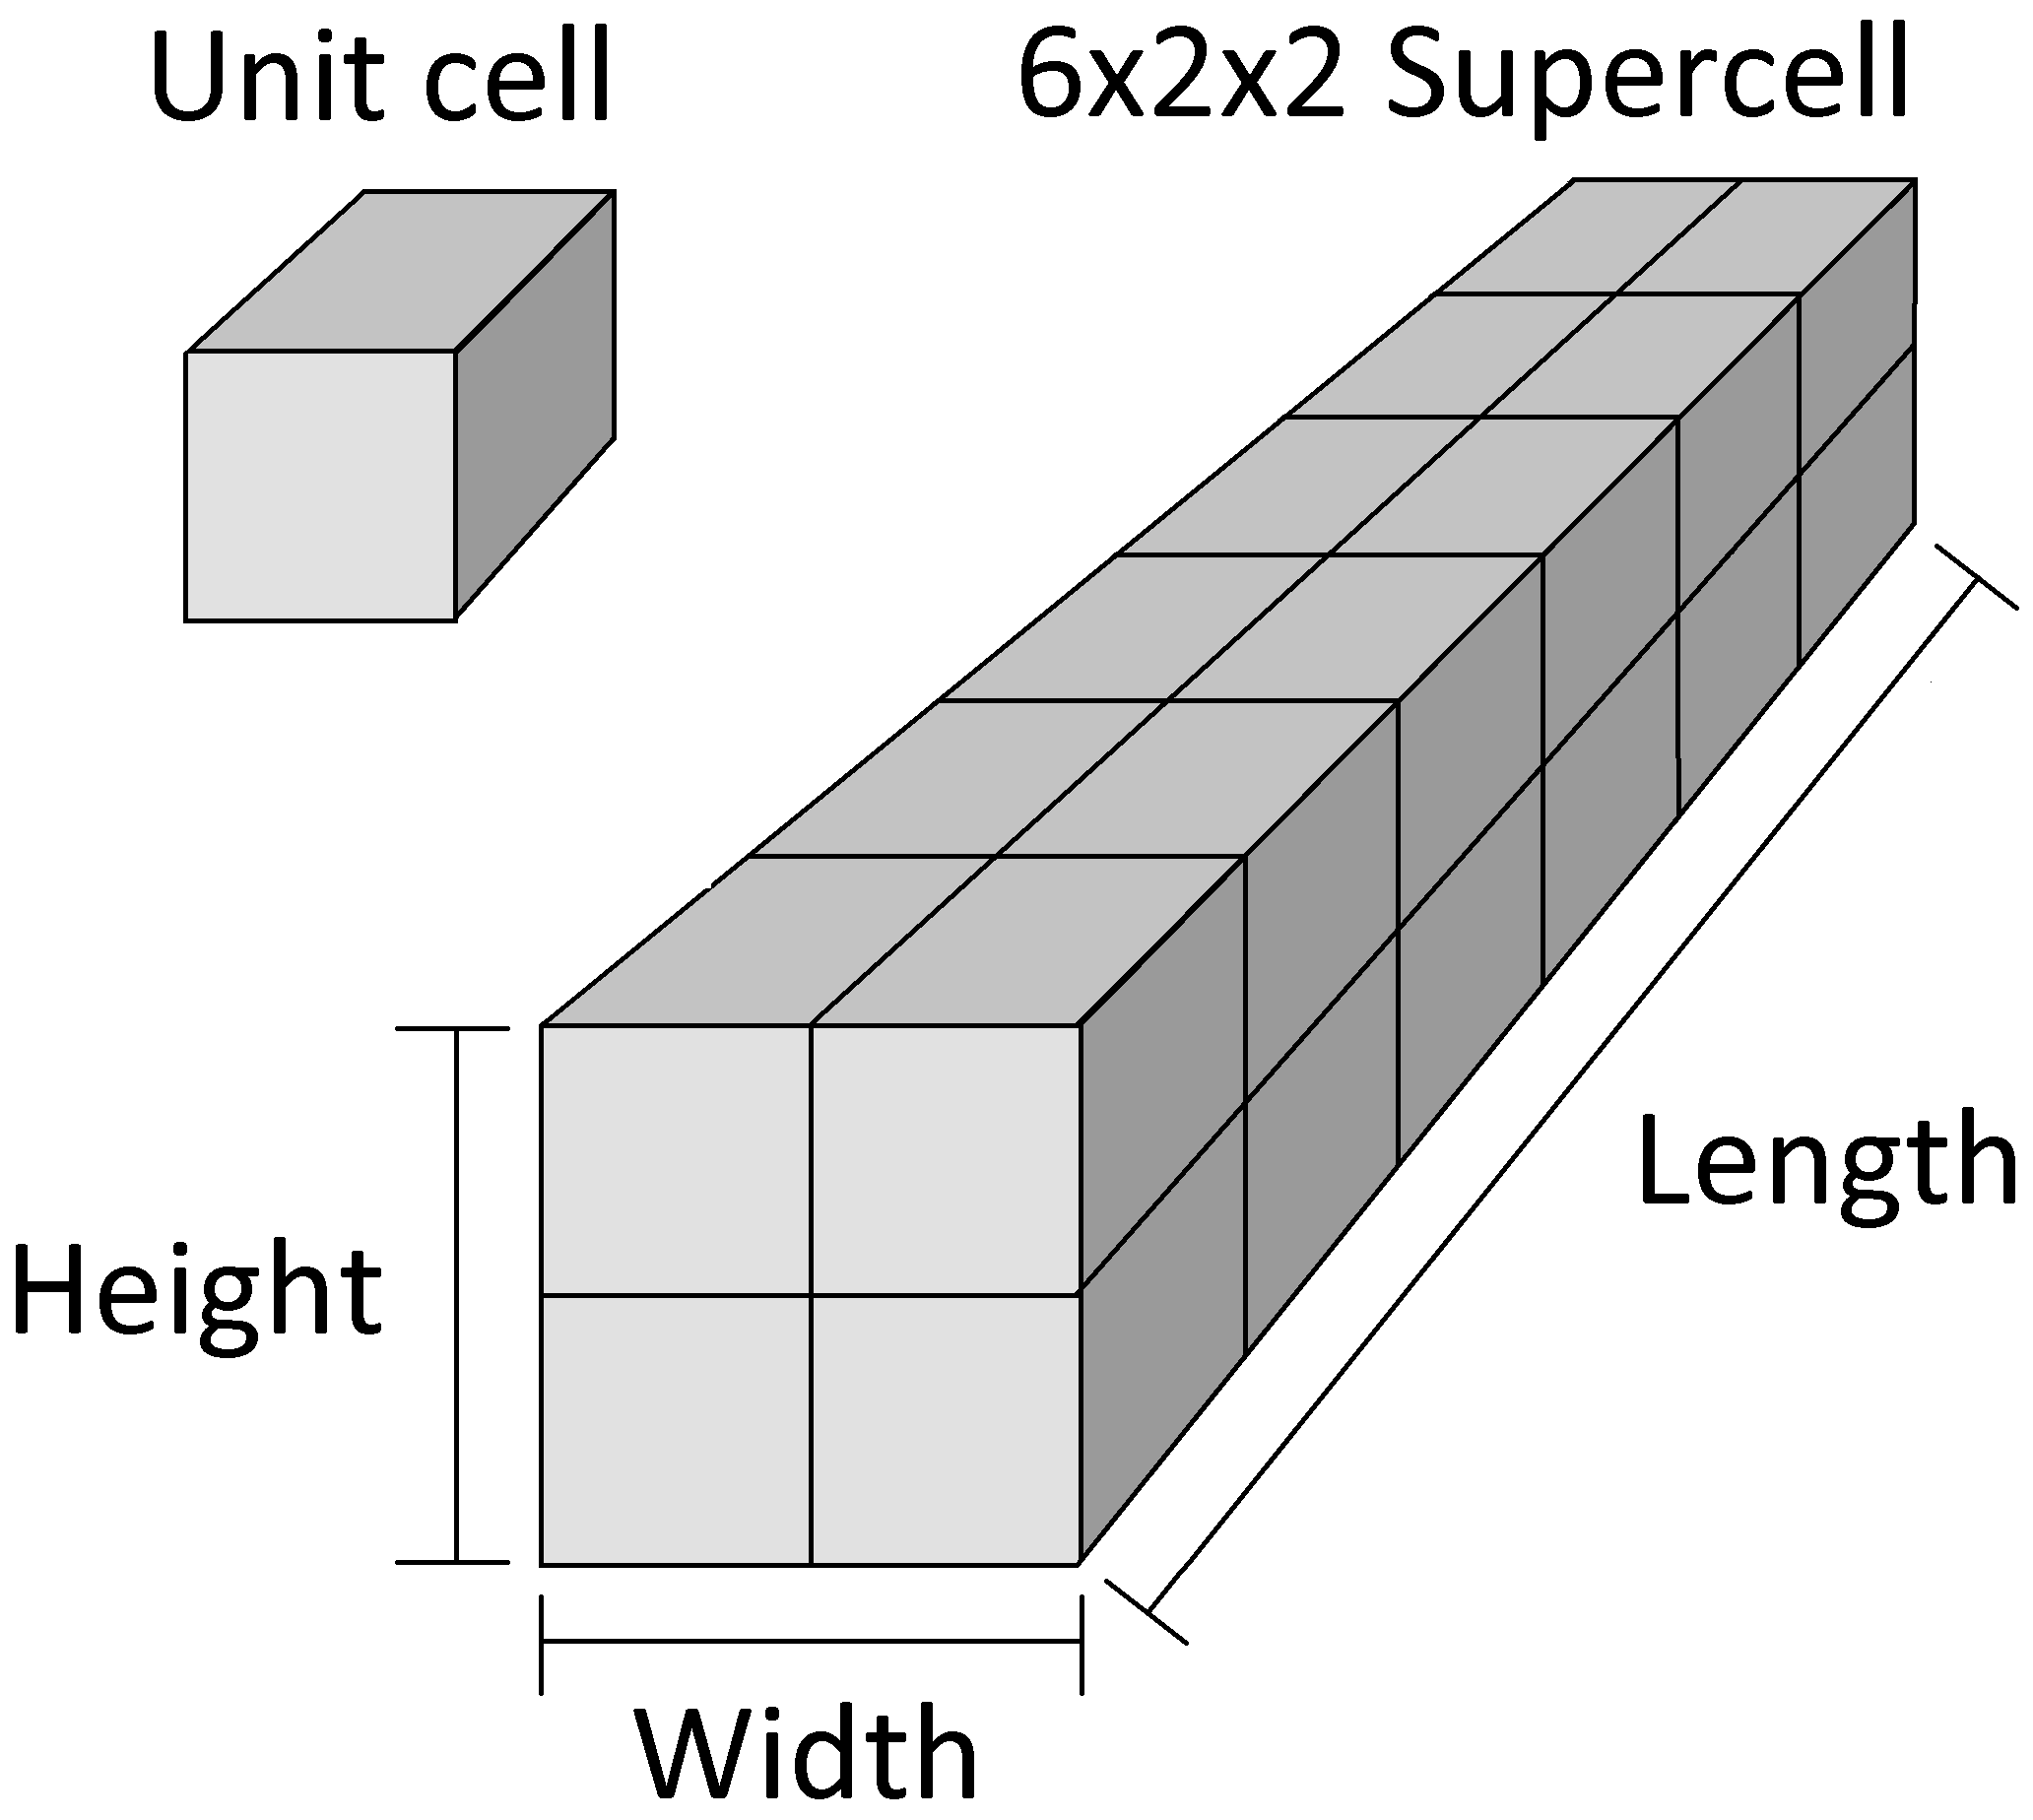
\includegraphics[width=\linewidth]{Figures/cell_diagram.png}
  \caption{The unit cell represents the smallest box of atoms that can be replicated to produce a crystal structure. A supercell is an arrangement of unit cells.}
  \label{fig:cell_dia}
\end{figure}

\begin{figure}[h]
  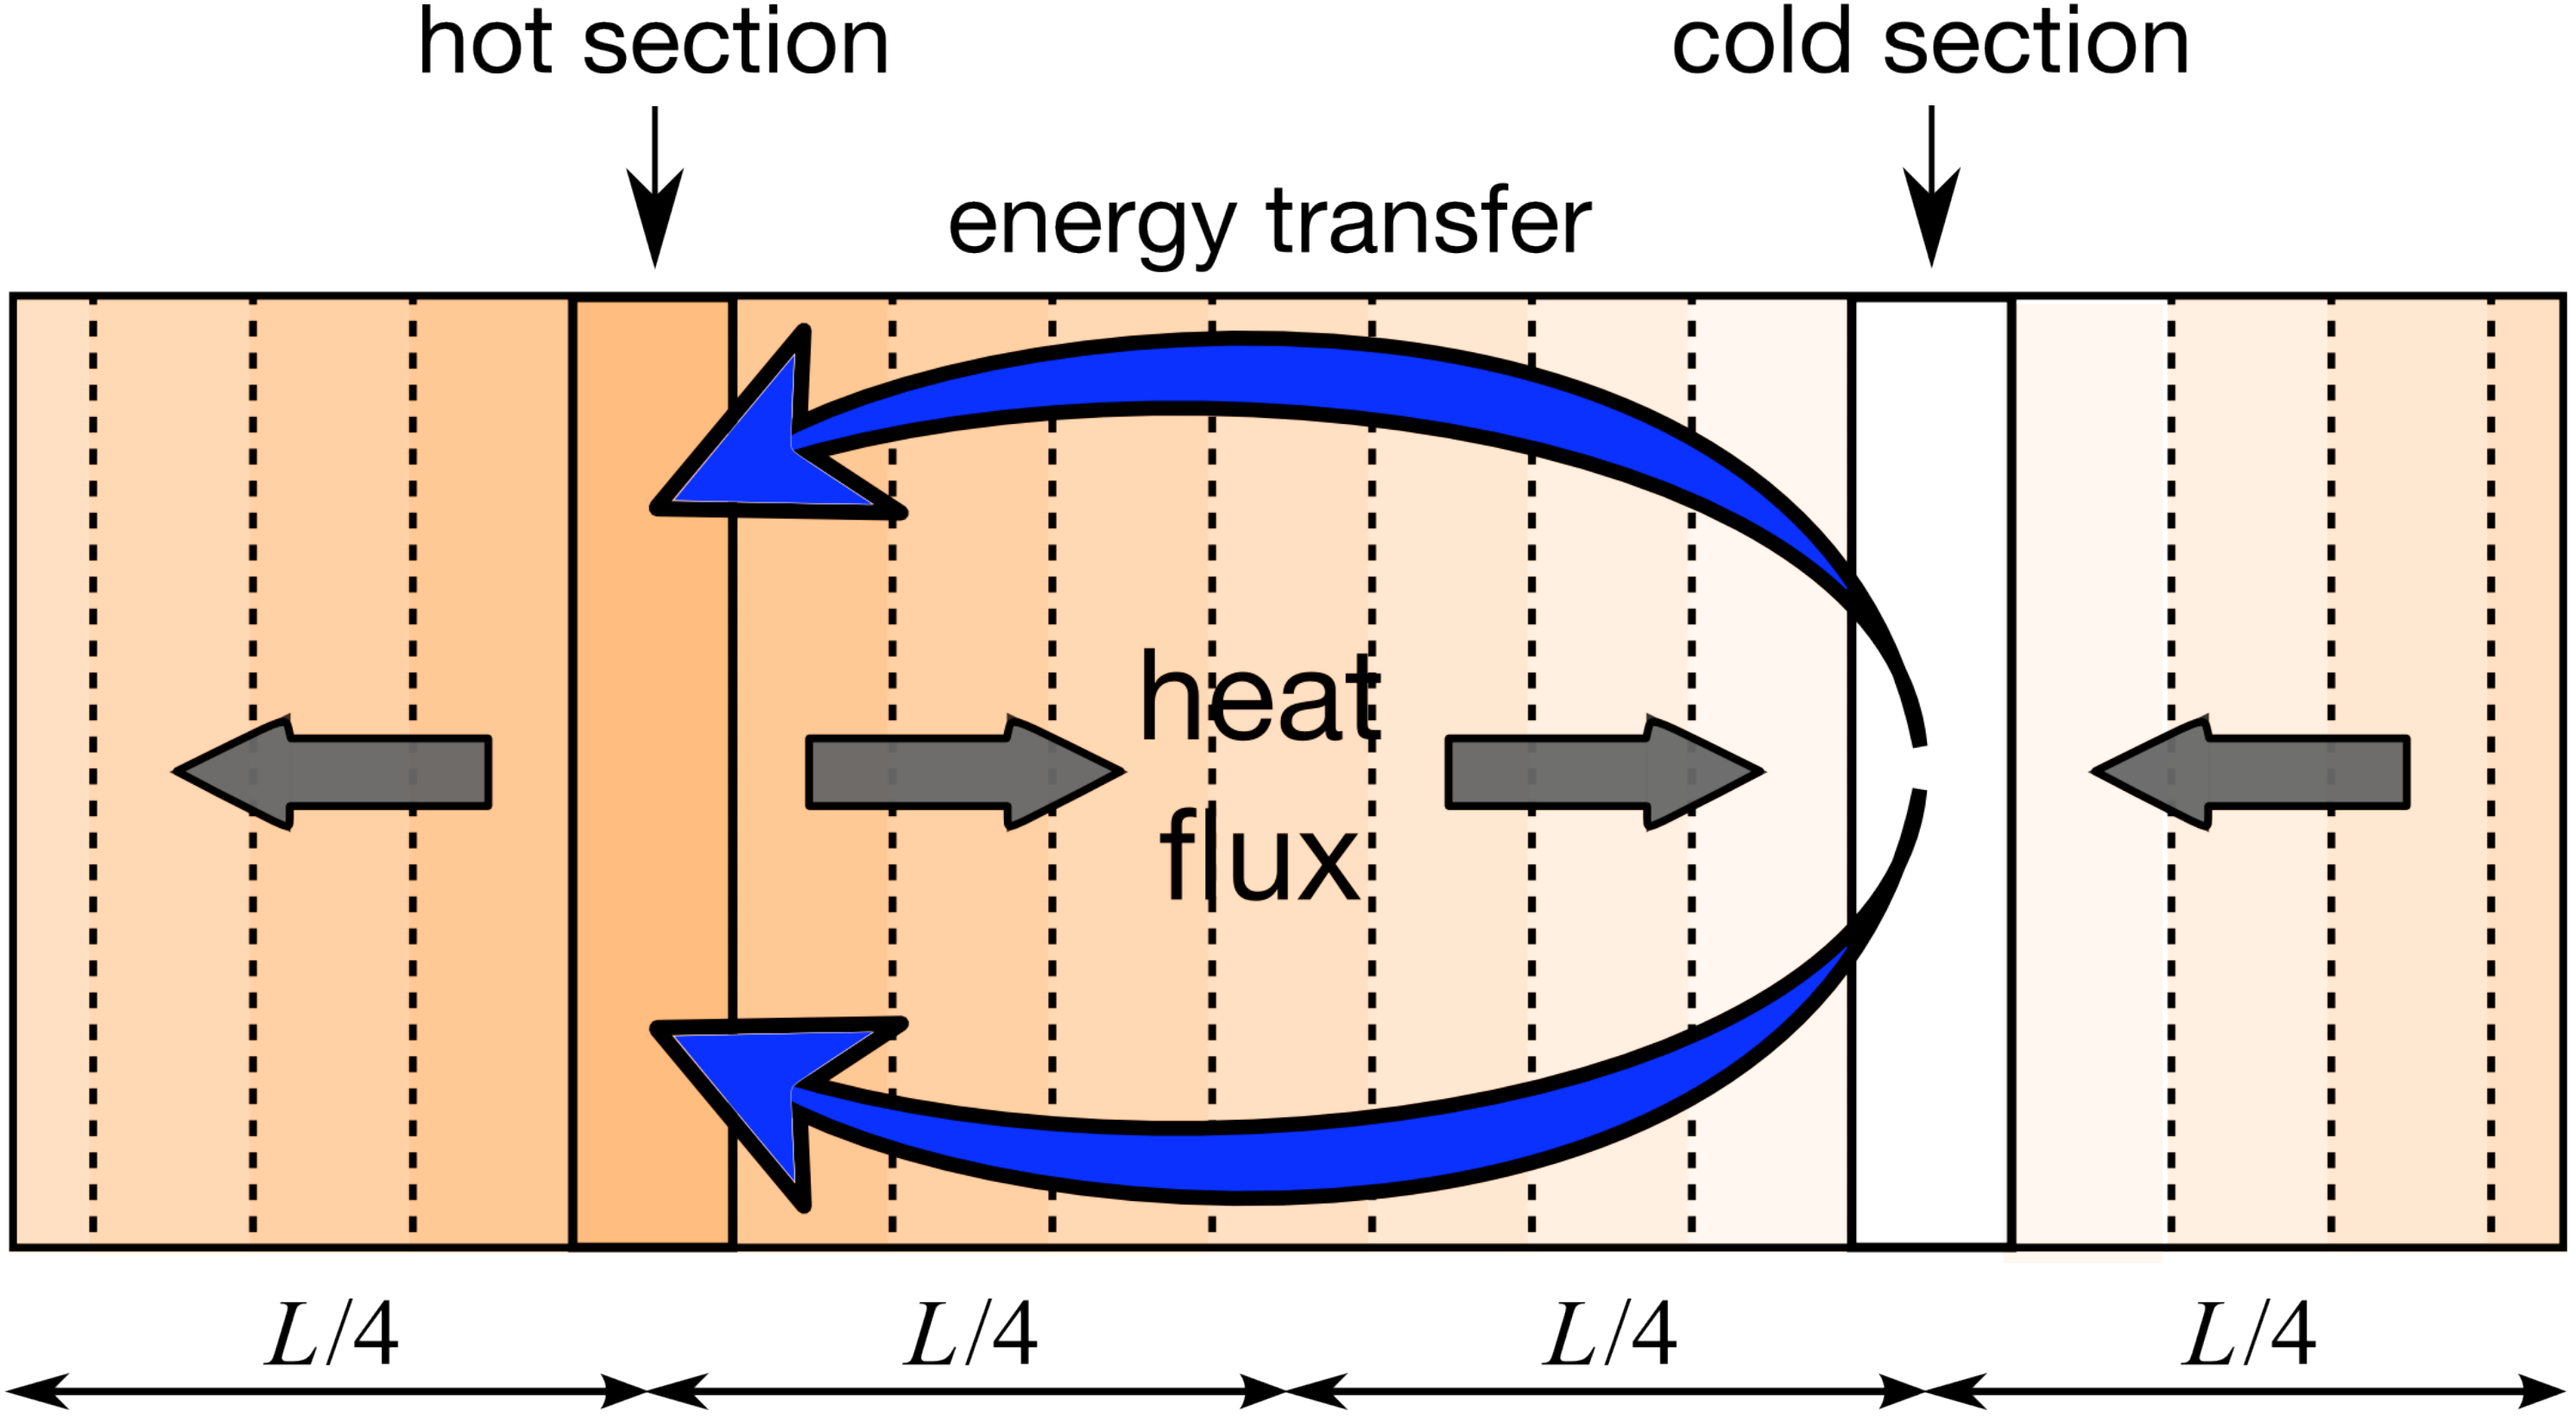
\includegraphics[width=\linewidth]{Figures/ss_direct_mod.png}
  \caption{Movement and distribution of heat in the direct method. Orange to white scale represents temperature \citep[modified from][]{Stackhouse2015}.}
  \label{fig:ss_direct}
\end{figure}



%-------------------
\subsubsection{Data processing}
%-------------------

In the immediate vicinity of hot and cold regions, the temperature gradient exhibits non-linear behaviour (INSERT FIGURE) due to the non-Newtonian nature of the heat exchange. Care must be taken to measure the linear portion, which is located roughly in the middle third of the temperature gradient. 

The finite size of the simulation cell truncates the mean free path, underestimating conductivity compared to that of the bulk material ($k_\infty$). Using results from simulations of varying cell length ($L$), conductivity is extrapolated to a length-independent value (where $b$ is a material dependent parameter),
%
\begin{equation}
{k_{L}}^{-1} = b L^{-1} + {k_{\infty}}^{-1}\ . 
\label{linear-extrap}
\end{equation}
%
Inverse conductivities from direct method simulations are plotted against corresponding inverse cell lengths. A straight line is fit to the data and extrapolated to the y-axis (at which the inverse cell length equals zero and real length equals infinity), where the intercept gives the inverse of the bulk material conductivity \citep{Schelling2002}.

\begin{figure}[h]
  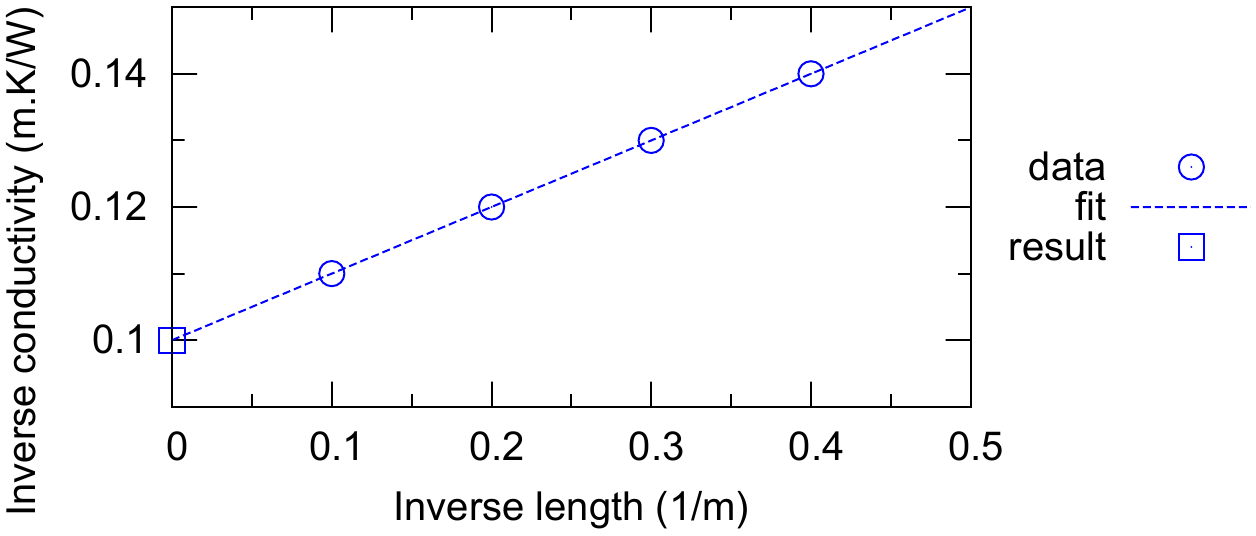
\includegraphics[width=\linewidth]{Figures/ideal_extrap.png}
  \caption{Idealised example of linear extrapolation procedure. Inverse computed conductivities are plotted against inverse simulation lengths. Extrapolation to y-axis gives conductivity of an infinite system length, i.e. the bulk material.}
  \label{fig:ideal}
\end{figure}



%-------------------
\subsubsection{Finite-size effects}
%-------------------

From kinetic theory [[[REF?]]], conductivities computed by the direct method ($k_L$) are dependent on length of simulation cell,
%
\begin{equation}
k_{L} = \frac{1}{3} C_{V} v l_{L}\ ,
\label{length-dep}
\end{equation}
%
where $C_v$ is the volumetric heat capacity, $v$ is the average phonon drift velocity, and $l_L$ is the phonon mean free path. 

Problems arise when the data do not support the aforementioned linear trend. There are two effects of finite system size that can cause an individual direct method simulation to diverge away from an inferred/expected linear trend, both of which result in overestimation of the length-dependent conductivity data point. First, when the distance between hot and cold sections (controlled by cell length) is shorter than the MFP, phonons travel ballistically (i.e. without any scattering events) from heat source to sink \citep{Sellan2010}. Conductivites in shorter length cells are overestimated when this occurs, reducing the gradient of the linear fit and thus underestimating the extrapolated conductivity.

For a given length, conductivity is dependent on the CSA, or aspect ratio of the simulation cell. Conductivity is overestimated due to an underestimation of phonon-phonon scattering, from sparse phonon phase sampling in cells where cross-section is small compared to length. Phonons that aren't resolved cannot contribute to phonon-phonon scattering effects. Reduced scattering means heat transport is artificially more efficient than expected from the bulk material. 

[[[SPECIFIC ALERT, REFERENCING THINGS I FOUND]]] However, the required CSA to abate this FSE is length-dependent. When the CSA is smaller than required for all cell lengths (e.g. 1x1 [FIGURE]), all conductivities are overestimated \citep{Thomas2010}. As the CSA is increased, the data points (and thus also the extrapolated result) shift to lower conductivities (higher inverse conductivities). It is at this point that the short cells with lengths of similar order, will report conductivities converged with respect to CSA. Assuming these cells are sufficiently long to avoid the ballistic phonon transport (BPT), a linear fit can be extrapolated to obtain conductivity (for CSA around 2x2, the case at 4000~K). 

The convergence is not necessarily observed concurrently for longer cells however, where they may show overestimated conductivities compared to the fit through short cells (\cite{Hu2011}). This would cause the fit to all data to be steeper than it should, increasing the extrapolated result.  [[[HOPEFULLY THIS IS TRUE]]] I can show that increasing CSA does not change the converged conductivities at short lengths, but does reduce values from longer cells and bring them into alignment with the expected fit. By comparing results with the Green-Kubo method, we will constrain the cell lengths in the linear extrapolation region to mitigate these effects.



%%%MOVE TO 3

%[[[SPECIFIC ALERT, REFERENCING THINGS I FOUND]]] The effect of FSE on conductivity results depends on the magnitude of conductivity/phonon MFP/physical conditions. At low kappa/low MFP/high T/ (my 4000~K), no BPT is observed, and short cells (>16 unit cells) can be used for extrapolation. In fact, short cells must be used to extrapolate, unless CSA considersations are made to ensure convergence of long cell results.
%[[[SPECIFIC ALERT, REFERENCING THINGS I FOUND]]] At high kappa/high MFP/low T (my 1000~K), BPT must considered at the shorter cells (just 6?). Effectively there is a "sweet-spot", a window of cell lengths for a given CSA that produce consistently-converged results. Long cells outside of the window require a larger CSA, short cells outside show BPT. At 4000~K the lower limit of the window is smaller than the minimum cell length considered, and the upper limit is between 16-24 unit cells. For 1000~K the lower limit of the window moves inside the simulated cell length range around 6-8 unit cells (OR MORE?). The upper limit of the window appears to be larger than 96 unit cells, including all long cells up to this value produces an extrapolation in agreement with GK.
%We have investigated this effect by varying CSA for a range of cell lengths, extrapolated conductivity decreases and eventually converges with CSA. We will use the smallest area that produces the converged conductivity for computational efficiency. 











%---------------------------------------
\subsection{Green-Kubo}
%---------------------------------------

Equilibrium molecular dynamic (EMD) simulations consider systems with constant average temperatures, and an overall heat flux of zero. The Green-Kubo method is an example of EMD, looking at heat flux caused by temperature flucuations in a simulation cell of roughly cubic dimensions. The lattice thermal conducivity of the system is related to the duration of these variations. I will use the Green-Kubo method to compute, but also to validate direct method results and workflow.	While the direct method has complex finite-size effects based on length and cross-sectional area, Green-Kubo is simpler in that number of atoms is the main factor. As long as the system is big enough, there is no need to care about arranging the cells or extrapolation procedures.

%-------------------
\subsubsection{Methodology}
%-------------------

The Green-Kubo method uses auto-correlation functions (ACFs) to quantify time-dependence of heat fluxes (shown in Figure~\ref{fig:gk_acf}, and Equation \ref{acf-j}). Instantaneous heat fluxes can be used to determine how energy is dissipated within a system, where brief flux events mean heat is transferred quickly indicating high thermal conductivity [[[and vice versa, BUT IS THIS TRUE?]]]. HIGHER CONDUCTIVITY, LONGER CORRELATION TIME. BRIEF FLUX EVENTS MEAN MORE DAMPING TO KILL SIGNAL. LONG CORRELATION, RESONANT SYSTEM, RINGING EFFECT, MORE EFFICIENT HEAT TRANSFER.

\begin{figure}[h]
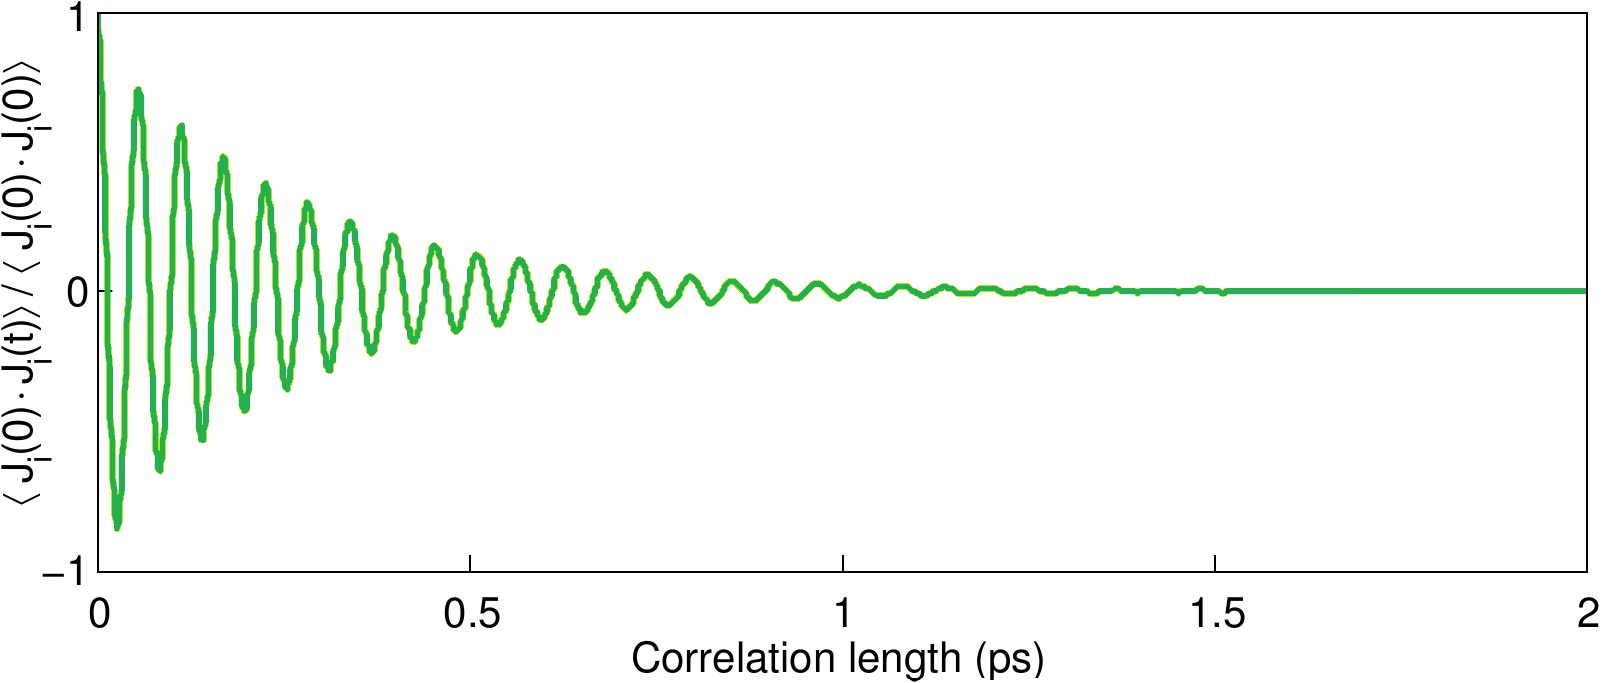
\includegraphics[width=\linewidth]{Figures/gk_acf.png}
\caption{Normalised ACF. Correlation is taken over a longer length than shown on this plot (100 ps), however the function decays to less than 1\% of its initial value at 2~ps. It continues to oscillate about zero, with a positive average value.}
\label{fig:gk_acf}
\end{figure}

The heat flux data required to generate the ACF is obtained from MD simulation in the NVE regime. As always, it is necessary to perform the NPT cell size convergence, and preliminary NVT to populate the atomic velocities.

The auto-correlation is obtained over the series of net heat flux in each crystallographic direction, for a timescale up to a chosen correlation length. 
~
\begin{equation}
ACF_i = \left \langle J_i(0) \cdot  J_i(t) \right \rangle,
\label{acf-j}
\end{equation}
~
where $i$ specifies direction, $J$ is heat flux, and $t$ is the correlation length. This acts as a cut-off, the significance of correlating points far apart in time decreases with the separation. The correlation length could be as long as the simulation length, but for large time differences there would be fewer and fewer heat flux pairs. This means there would be increased uncertainty on points of decreasing relevance. The correlation lengths I use are much shorter than the simulation length.  

The integral of heat flux ACF is proportional to thermal conductivity via the Green-Kubo equation (see Figure~\ref{fig:gk_int} and Equation \ref{gk-int}), 
~
\begin{equation}
\kappa_i = \frac{V}{k_{B}T^{2}} \int_{0}^{\infty} \left \langle J_i(0) \cdot  J_i(t) \right \rangle dt ,
\label{gk-int}
\end{equation}
~
[[[I am using ``k''s and ``kappa''s to represent \tc, kappa here and k earlier?]]] where $V$ is the simulation cell volume, $k_B$ is the Boltzmann constant, and $T$ is the average temperature of the system. In this study we use Green-Kubo results as an independent check on the direct method, as they do not have the same finite size-effects. Obtaining a converged conductivity result simply depends on using a large enough cell volume / number of atoms. 

\begin{figure}[h]
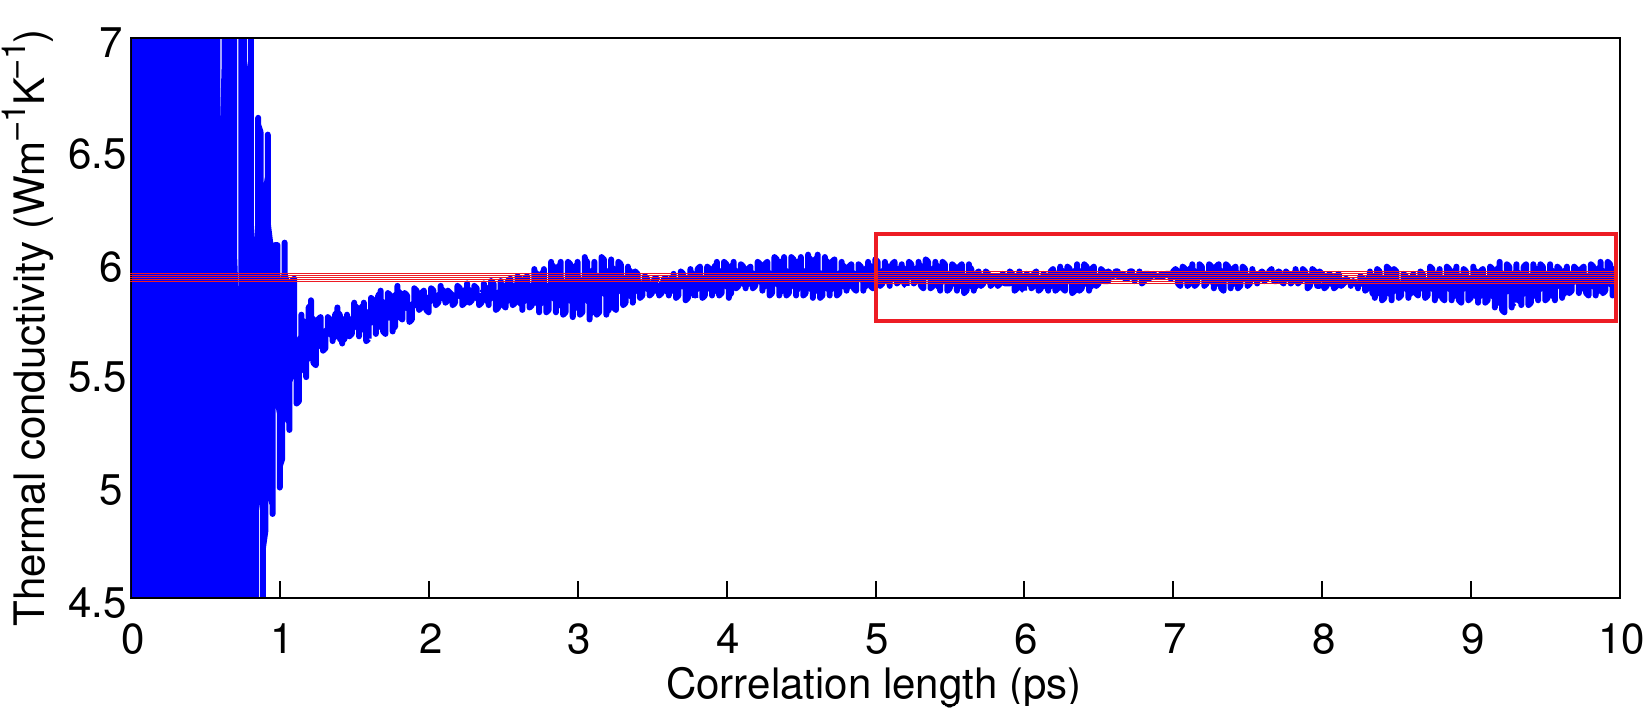
\includegraphics[width=\linewidth]{Figures/gk_int.png}
\caption{Integrated ACF, multiplied by constants to get thermal conductivity. Large variation in the first 1 ps corresponds to the correlation time where the ACF is unconverged (still decaying / large oscillations). Thermal conductivity is averaged from correlation time of 5~--~10~ps (region in red box).}
\label{fig:gk_int}
\end{figure}





%-------------------
\subsubsection{Data processing}
%-------------------

The individual integrals obtained from the Green-Kubo show variation from the average combined integral on the order of the mean. Many simulations from different intital temperature conditions are required in order to ensure good sampling of conductivity, as well as ensuring the computation time for each is long enough for convergence. This makes Green-Kubo a computationally expensive method, especially for large systems.

From a large sample of integrals, the mean integral is examined to find a time window of convergence. This region exists after the inital large variations, and before any drift behaviour. This correlation window is then applied to all integrals seperately, yielding a population of conductivities and uncertainties. I then applied a weighted average to this information, obtaining a conductivity for the entire population.

The ACF should decay to zero as correlation time tends to infinity, however noise in the ACF prevents this. This will ultimately cause the integral to diverge/drift on long timescales. \citet{Howell2012} fits a series of exponential decays to their ACF, forcing the expected decay to zero and subsequent (constant) integral convergence. This is represents a significant improvement on the conductivity estimate at long correlation lengths, but is mostly similar with the un-fit integrals early in the correlation. (INTEGRAL DRIFT FIGURE, JUST THE ONE INTEGRAL FOR 100PS)

!!! (STACKHOUSE 2010 REFERENCES Volz and Chen 2000; Sun and Murthy 2006)







%-----------------------------------------------------------
\section{Previous work}
%-----------------------------------------------------------

%---------------------------------------
\subsection{Method comparison}
%---------------------------------------

A wealth of data comparing the conductivities yielded by non-equilibrium and equilibrium molecular dynamics is available for silicon, at temperatures around 1000~K. \citet{Schelling2002} consider Sillinger-Weber silicon, and find good agreement in conductivity results, once FSE are addressed. \citet{Sellan2010} consider the same material and find the two methods don't agree at a lower temperature of 500~K, although it is agrued by \citet{Howell2012} that there direct method finite-size scaling was inappropriate. \citeauthor{Howell2012} performs their own calculations and review of literature, finding consistent results between the methods and the suite of studies considered. \citet{Wang2017} contribute further results consistent with \citeauthor{Howell2012} for SW Si at 1000~K, as well showing agreement between methods for graphene and silicene at 300~K. 

\citet{Dong2018} show consistency between NEMD and EMD for silicene and Si nanowires. \citet{Turney2009} show very coherent agreements for Lennard-Jones argon across a range of simulation methods, including NEMD, EMD Green-Kubo, along with Boltzmann transport equation and lattice dynamics approaches. None of these studies consider a material as complicated as \bdgs however, of which I will show the equivalence (or lack thereof) of computed conductivity between the direct and Green-Kubo methods.

%---------------------------------------
\subsection{Bridgmanite FSE}
%---------------------------------------

As introduced earlier, \citet{Ammann2014} used NEMD to calculate the thermal conductivity of \bdg. For conditions of 20~GPa and 2000K, they observe convergence with respect to cross-sectional area (CSA) with dimensions of 2$\times$2 unit cells (UC), irrespective of crystallographic direction. They only consider cell lengths up to 32 unit cells however, which means they may be missing the effect understimated phonon-phonon scattering for a small CSA. Their extrapolation is not incorrect for the results that they have (see their Figure 3), but the gradient can be seen to decrease when 3$\times$3 CSA is considered. The computed conductivity of cells over 20~UC decreases as this area increases, possibly due to increased phonon-phonon scattering effect. I will investigate this further by studying longer systems with larger CSAs.

!!! ALSO CONSIDER STACKHOUSE 2015?



%-----------------------------------------------------------
\section{Conclusion}
%-----------------------------------------------------------

In this chapter I introduced atomic-scale modelling, how it can be performed, and how atoms can be made to behave like realistic materials. I outline molecular dynamics methodologies for computing thermal conductivity, and potential problems associated with them. In the following chapter I will apply these techniques to study the effects of finite simulation size on computed \bdgs conductivity result. I will use and compare both of the techniques, as they have independent finite-size effects (FSE).

Once the methodology is checked to have minimized FSE, I will calculate how temperature and composition affect \bdgs conductivity at CMB conditions. This will feed into calculations of lower mantle heat flux, and how thermo-and/or-chemical piles, the large low shear velocity provinces (LLSVPs), influence lateral variations therein. This will be compared with observed shear wave velocity reductions to offer insight into the extend of LLSVP temperature and chemical heterogeneity.



%%-------------------
%\subsubsection{Parameter drift/convergence}
%%-------------------
%We ensure all calculations are run for a sufficient length of time for the conductivity value to converge. When conductivity fails to converge it means either the simulations needs to be run for longer (unlikely with our nanosecond-scale classical calculations), or the system temperature has drifted. When NVE simulations are run for a long time there is noticable drift in the average system temperature (due to numerical approximations in the equation of motion), which in turn causes drift in the computed conductivity.

%NPT-NVT-NVE PROCESS



